\providecommand{\main}{../../..}
\documentclass[\main/main.tex]{subfiles}
\begin{document}

\subsection{Esercizio 6}
Un macchinario comincia a mostrare segni di usura. Si stima che, senza interventi di manutenzione, possa funzionare ancora per 3 mesi. L'intervento di manutenzione consentirebbe di usarlo ancora per un anno, ma presenta dei rischi: c'`e una probabilità del 30\% che danneggi definitivamente il macchinario. Si descriva il problema con un albero di decisione, assumendo come funzione di utilità la durata residua del macchinario.

Si risolva il problema con l'albero di decisione applicando il criterio del caso pessimo.

Si ripeta la risoluzione con il criterio del valore atteso, commentando brevemente le differenze rispetto all'altro procedimento (se ve ne sono).

Si supponga che un test consenta di ottenere informazioni sullo stato del macchinario, e quindi di prevedere (con qualche incertezza) l'esito dell'intervento: se il macchinario è destinato a sopravvivere al test, questo ha esito positivo nel 90\% dei casi; se il macchinario è destinato a soccombere, il test ha esito negativo nell'80\% dei casi. Si risolva il problema di decidere se eseguire o no il test e se eseguire o no l'intervento di manutenzione.
Si può esprimere quantitativamente il valore dell'informazione fornita dal test? Se sì, in che modo?

\subsection{Soluzione esercizio 6}
\subsubsection*{Albero di decisione}
\begin{figure}
  \begin{tikzpicture}
    \Tree[.root
    [.riparo [.$0.3$ $0m$ ][.$0.7$ $12m$ ]]
    [.\text{non riparo} [$3m$ ]]
    ]
  \end{tikzpicture}
\end{figure}

\subsubsection*{Caso pessimo}
\begin{figure}
  \begin{tikzpicture}
    \Tree[.root
    [.riparo [$0m$ ]]
    [.\text{non riparo} [$3m$ ]]
    ]
  \end{tikzpicture}
\end{figure}
Secondo il criterio del caso pessimo, in cui scelgo il peggiore risultato possibile, scelgo di non riparare il macchinario.

\subsubsection*{Caso valore atteso}
\begin{figure}
  \begin{tikzpicture}
    \Tree[.root
    [.riparo [$8.4m$ ]]
    [.\text{non riparo} [$3m$ ]]
    ]
  \end{tikzpicture}
\end{figure}

Secondo il criterio del caso medio, con cui peso ogni utilità per la sua probabilità, scelgo di riparare il macchinario.

\subsubsection*{Caso con test}
Effettuare il test mi garantisce un'utilità, ottenuta tramite il criterio del caso medio, di $8.49$ maggiore di quella massima ottenuta senza effettuare il test di $8.4m$.

\begin{table}
  \begin{tabular}{|c|c|c|c|c|c|}
    \hline
    esito          & percentuale & utilità seguendo test & riparo ignorando test & non riparo ignorando test \\
    \hline
    positivo       & 63\%        & $12m$: riparo         & $12m$                 & $3m$                      \\
    \hline
    falso negativo & 7\%         & $3m$: non riparo      & $12m$                 & $3m$                      \\
    \hline
    negativo       & 24\%        & $3m$: non riparo      & $0m$                  & $3m$                      \\
    \hline
    falso positivo & 6\%         & $0m$: rompo           & $0m$                  & $3m$                      \\
    \hline
    \hline
    Totale         &             & $8.49m$               & $8.4m$                & $3m$                      \\
    \hline
  \end{tabular}
\end{table}

\subsubsection*{Utilità del test}
L'utilità del test è quantificabile come la differenza tra l'utilità derivata dal caso in cui viene eseguito e nel caso in cui esso non venga eseguito, quindi qui $0.09m$.

\end{document}
